% 原卷第20题三棱柱及平面 EB_1C_1F；不标注未出现在原图中的体积区域名。
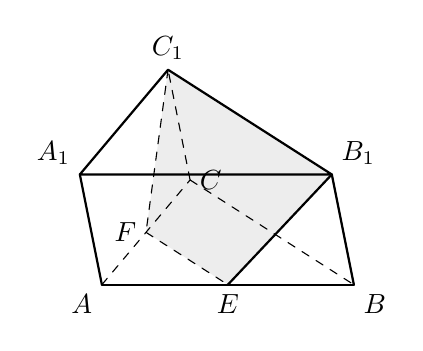
\begin{tikzpicture}[x=0.8cm,y=0.7cm,line cap=round,line join=round]
  \coordinate (A) at (0,0);
  \coordinate (B) at (4,0);
  \coordinate (C) at (1.4,1.9);
  \coordinate (Aone) at (-0.35,2.0);
  \coordinate (Bone) at (3.65,2.0);
  \coordinate (Cone) at (1.05,3.9);
  \coordinate (E) at (2,0);
  \coordinate (F) at (0.7,0.95);
  \fill[gray!14] (E)--(Bone)--(Cone)--(F)--cycle;
  \draw[thick] (A)--(B);
  \draw[thick] (Aone)--(Bone)--(Cone)--(Aone);
  \draw[thick] (A)--(Aone) (B)--(Bone);
  \draw[dashed] (A)--(C) (C)--(Cone) (C)--(B) (Cone)--(F) (F)--(E);
  \draw[thick] (E)--(Bone);
  \node[below left] at (A) {$A$};
  \node[below right] at (B) {$B$};
  \node[right] at (C) {$C$};
  \node[above left] at (Aone) {$A_1$};
  \node[above right] at (Bone) {$B_1$};
  \node[above] at (Cone) {$C_1$};
  \node[below] at (E) {$E$};
  \node[left] at (F) {$F$};
\end{tikzpicture}
